\documentclass[a4paper]{article}

% LTeX: enabled=false
% Kodiranje in podpora slovenščini
\usepackage[T1]{fontenc}        % kodiranje znakov v .pdf
\usepackage[slovene]{babel}

\usepackage{fontspec}
\usepackage{lualatex-math}
\usepackage{unicode-math}

% \setmainfont{TeX Gyre Pagella}
% \setmathfont{TeX Gyre Pagella Math}
\setmathfont{Latin Modern Math}
\setmathfont{Asana Math}[range={scr}]
\setmathfont{STIX Two Math-Regular}[range={bb}]
% \setmathfont{Asana Math}[range={"007B,"007D}]  % {}
\setmathfont{Asana Math}[range={8709, \setminus}]  % U+2205, emptyset


% \usepackage{concrete}           % pisave po okusu Donalda Knutha

% Ta paket potrebujemo, ker amsart spreminja male črke v velike v naslovu,
% in tega ne zna pravilno delati s šumniki. Paket textcase ta problem odpravi.
% Glej: https://tex.stackexchange.com/questions/211305/problem-with-greek-title
\usepackage{textcase}

% Paketi za matematiko

\undef\eth
\undef\digamma
\undef\backepsilon
\usepackage{amsmath}  % razna okolja za poravnane enačbe ipd.
\usepackage{amsthm}   % definicije okolij za izreke, definicije, ...
% \usepackage{xypic}    % paket za diagrame

% \usepackage{mathtools}


\usepackage{fancyhdr}
\usepackage{extramarks}
\usepackage{enumerate}
\usepackage{tikz}
\usetikzlibrary{babel}
% \usepackage[plain]{algorithm}
% \usepackage{algpseudocode}
% \usepackage{listings}
\usepackage{minted}
\usepackage{hyperref}

\usetikzlibrary{cd,positioning}

%
% Basic Document Settings
%

\topmargin=-0.45in
\evensidemargin=0in
\oddsidemargin=0in
\textwidth=6.5in
\textheight=9.0in
\headsep=0.25in
\headheight=12.5pt

\linespread{1.1}

\pagestyle{fancy}
\lhead{\hmwkAuthorName}
\chead{\hmwkClass:\ \hmwkTitle}
\rhead{\firstxmark}
\lfoot{\lastxmark}
\cfoot{\thepage}

\renewcommand\headrulewidth{0.4pt}
\renewcommand\footrulewidth{0.4pt}

\setlength\parindent{0pt}

%
% Create Problem Sections
%

\newcommand{\enterProblemHeader}[1]{
    \nobreak\extramarks{}{Naloga \arabic{#1} se nadaljuje na naslednji strani\ldots}\nobreak{}
    \nobreak\extramarks{Naloga \arabic{#1} (nadaljevanje)}{Naloga \arabic{#1} se nadaljuje na naslednji strani\ldots}\nobreak{}
}

\newcommand{\exitProblemHeader}[1]{
    \nobreak\extramarks{Naloga \arabic{#1} (nadaljevanje)}{Naloga \arabic{#1} se nadaljuje na naslednji strani\ldots}\nobreak{}
    \stepcounter{#1}
    \nobreak\extramarks{Naloga \arabic{#1}}{}\nobreak{}
}

\setcounter{secnumdepth}{0}
\newcounter{partCounter}
\newcounter{solCounter}
\newcounter{homeworkProblemCounter}
\setcounter{homeworkProblemCounter}{1}
\nobreak\extramarks{Naloga \arabic{homeworkProblemCounter}}{}\nobreak{}

%
% Homework Problem Environment
%
% This environment takes an optional argument. When given, it will adjust the
% problem counter. This is useful for when the problems given for your
% assignment aren't sequential. See the last 3 problems of this template for an
% example.
%
\newenvironment{homeworkProblem}[1][-1]{
    \ifnum#1>0
        \setcounter{homeworkProblemCounter}{#1}
    \fi
    \section{Naloga \arabic{homeworkProblemCounter}}
    \setcounter{partCounter}{1}
    \setcounter{solCounter}{1}
    \enterProblemHeader{homeworkProblemCounter}
}{
    \exitProblemHeader{homeworkProblemCounter}
}


%
% Title Page
%

\title{
    \vspace{2in}
    \textmd{\textbf{\hmwkClass:\ \hmwkTitle}}\\
    \normalsize\vspace{0.1in}\small{Rok\ oddaje\ \hmwkDueDate}\\
    % \vspace{0.1in}\large{\textit{\hmwkClassInstructor\ \hmwkClassTime}}
    \vspace{3in}
}

\author{\hmwkAuthorName}
\date{}

% \renewcommand{\part{}}[1]{\textbf{\large Part \Alph{partCounter}}\stepcounter{partCounter}\\}
\renewcommand{\part}{
    \vspace{10pt}
    \textbf{(\alph{partCounter})}
    \stepcounter{partCounter}
}

% Alias for the Solution section header
\newcommand{\solution}[1][*]{
    \vspace{10pt}
    \ifx#1*
        \textbf{Rešitev (\alph{solCounter})}
        \stepcounter{solCounter}
    \else
        \textbf{Rešitev}
    \fi
}

\newcommand{\example}{
    \vspace{10pt}
    \textbf{Primer:}\\
}

\renewcommand{\d}{\;\mathrm d}
% \newcommand{\vphi}{\phi}
\renewcommand{\phi}{\varphi}
\newcommand{\eps}{\varepsilon}
\renewcommand{\hat}{\widehat}
\renewcommand{\tilde}{\widetilde}
\renewcommand{\bar}{\overline}
\newcommand{\subs}{\subseteq}
\newcommand{\nin}{\not\in}

\newcommand{\p}[1]{\left( {#1} \right)}
\newcommand{\set}[2]{\left\{ #1 \mid #2 \right\}}
\newcommand{\newfrac}[2]{{}^{#1}\!/_{\!#2}}
\newcommand{\quot}[2]{\newfrac{#1}{#2}}
\DeclareMathOperator{\im}{im}
\DeclareMathOperator{\coker}{coker}
\DeclareMathOperator{\coim}{coim}
\DeclareMathOperator{\id}{id}
\newcommand{\mb}[1]{\mathbold{#1}}
\newcommand{\mf}[1]{\mathfrak{#1}}
\newcommand{\mc}[1]{\mathcal{#1}}
\newcommand{\cc}{\complement}

\newcommand{\bin}[2]{\mathrm{Bin}{\p{#1, #2}}}

\newcommand{\for}[2]{\forall#1.\;#2}
\newcommand{\exist}[2]{\exists\;#1\smallni:\;#2}
\newcommand{\existi}[2]{\exists!\;#1\smallni:\;#2}

\renewcommand{\check}{ \(\checkmark\)}

\makeatletter
\newcommand{\oset}[3][0ex]{%
  \mathrel{\mathop{#3}\limits^{
    \vbox to#1{\kern-2\ex@
    \hbox{$\scriptstyle#2$}\vss}}}}
\makeatother


\newcommand{\hmwkTitle}{Projektna naloga}
\newcommand{\hmwkDueDate}{9.~2022}
\newcommand{\hmwkClass}{Statistika}
\newcommand{\hmwkClassTime}{}
\newcommand{\hmwkClassInstructor}{}
\newcommand{\hmwkAuthorName}{\textbf{Strah},~27181100}

\begin{document}

\maketitle

\pagebreak

Vse naloge so rešene z orodjem Jupyter, ki kot jedro uporablja SageMath.
Za diagrame uporabljam matplotlib.

\begin{homeworkProblem}
    \solution
    \begin{minted}[autogobble,breaklines]{python}
        import numpy as np
        import matplotlib.pyplot as plt
        import csv
        import random

        with open('../data/Kibergrad.csv', 'r') as f:
            f.readline()
            reader = csv.reader(f)
            kibergrad = list(tuple(map(int, line)) for line in reader)

        kibergrad_by_square = tuple(list(filter(lambda x: x[4] == i+1, kibergrad)) for i in range(4))
        sample = tuple(random.choices(population=sq, k=100) for sq in kibergrad_by_square)
        plt.boxplot(x=tuple(list(e[3] for e in sq) for sq in sample))
        plt.show()
    \end{minted}
    \begin{figure}[h!]
        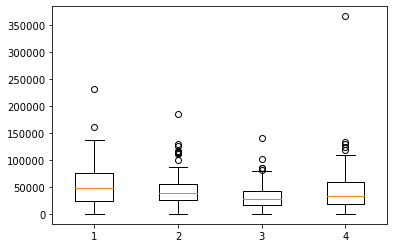
\includegraphics{fig-1-1.png}
    \end{figure}

    Sicer vidimo neke manjše razlike (dohodki so malce nižji v južni četrti in malce višji v severni), ampak menim, da četrti ne vplivajo bistveno na dohodek.

    \pagebreak
    \solution
    \begin{minted}[autogobble,breaklines]{python}
        sample2 = (sample[0], *(random.choices(population=kibergrad_by_square[0], k=100) for _ in range(4)))
        plt.boxplot(x=tuple(list(e[3] for e in sq) for sq in sample2))
        plt.show()
    \end{minted}
    \begin{figure}[h!]
        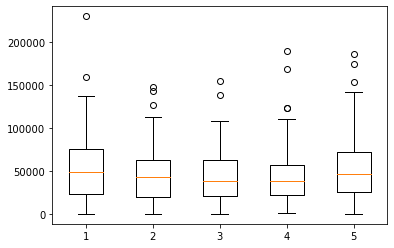
\includegraphics{fig-1-2.png}
    \end{figure}

    Graf zgleda približno kot zgornji, kar še bolj utemelji moje mnenje, da četrti ne vplivajo na dohodek.

    \solution
    \begin{minted}[autogobble,breaklines]{python}
        incomes_by_square = tuple(list(e[3] for e in sq) for sq in kibergrad_by_square)
        explained_var = np.var(list(np.mean(sq) for sq in incomes_by_square))
        residual_var = np.mean(list(np.var(sq) for sq in incomes_by_square))
        print(f"explained variance: {explained_var}\nresidual variance: {residual_var}")
    \end{minted}
    \begin{verbatim}
        explained variance: 8688785.712368913
        residual variance: 1027977659.8502393
    \end{verbatim}
    Kot vidimo, četrti res ne vplivajo bistveno na dohodek.

\end{homeworkProblem}

\newpage

\begin{homeworkProblem}
    \solution
    \begin{minted}[autogobble,breaklines]{python}
        import numpy as np
        import matplotlib.pyplot as plt
        import csv
        import random
        import math

        with open('../data/Palice.csv', 'r') as f:
            f.readline()
            reader = csv.reader(f)
            palice = list(int(line[1]) for line in reader)

        var('k')
        f(k, n, p) = (factorial(n)/factorial(k)/factorial(n-k)) * p^k * (1-p)^(n-k)
        l(p) = sum([log(f(k, 5, p))*(palice[k]) for k in range(6)])
        p_0 = solve(derivative(l) == 0, p)[0].right()
    \end{minted}
    Vrednost \(p₀\) je \(199/1400 ≈ 0.14\).

    \solution
    \begin{minted}[autogobble,breaklines]{python}
        palice2 = [157, 69, 35, 19]
        f_tail = f(3, 5, p_0) + f(4, 5, p_0) + f(5, 5, p_0)
        chi2 = sum([(palice2[k] - 280*f(k, 5, p_0))^2/f(k, 5, p_0) for k in range(3)]) + (19 - 280*f_tail)^2/f_tail
        chi2 /= 280
        print(N(chi2))
        print(N(exp(-chi2/2)))
    \end{minted}
    \begin{verbatim}
        44.1486610184320
        2.58964401605015e-10
    \end{verbatim}

    Ker je vrednost \(χ²\) velika lahko ničelno domnevo potrdimo.

    \pagebreak
    \solution
    Najprej izračunamo, za katere \(pᵢ\) je verjetje posameznega opažanja največje:
    \begin{minted}[autogobble,breaklines]{python}
        var('x')
        var('p')
        var('m')
        f(x, m, p) = (factorial(m)/factorial(x)/factorial(m-x)) * p^x * (1-p)^(m-x)
        S(x, m, p) = derivative(f(x, m, p), p)
        solve(S(x, m, p) == 0, p)
    \end{minted}
    \begin{verbatim}
        [p^x == x*(p - 1)*p^(x - 1)/(x - m)]
    \end{verbatim}
    Dobimo enačbo \(pᵢˣ = \frac{xᵢ}{mᵢ-xᵢ}(1-pᵢ)⋅pᵢ^{xᵢ-1}\), od koder sledi \(pᵢ=0 ∨ pᵢ = \frac{x}{m}\).

    Razmerje verjetij je potemtakem enako \(Λ = ∏ᵢ\frac{f₁ᵢ}{f₀ᵢ}\), kjer je 
    \begin{align*}
        f₀ᵢ &= \binom{mᵢ}{xᵢ} p^{xᵢ} (1-p)^{mᵢ-xᵢ}\\
        f₁ᵢ &= \binom{mᵢ}{xᵢ} pᵢ^{xᵢ} (1-pᵢ)^{mᵢ-xᵢ} = \binom{mᵢ}{xᵢ}mᵢ^{-mᵢ}xᵢ^{xᵢ}(mᵢ-xᵢ)^{mᵢ-xᵢ}\text{, če je \(xᵢ ≠ 0, mᵢ\) in \(1\) sicer}
    \end{align*}
    Potem je \(\frac{f₁ᵢ}{f₀ᵢ} = \left(\frac{pᵢ}{p}\right)^{xᵢ}\left(\frac{1-pᵢ}{1-p}\right)^{mᵢ-xᵢ} = mᵢ^{-mᵢ}\left(\frac{xᵢ}{p}\right)^{xᵢ}\left(\frac{mᵢ-xᵢ}{1-p}\right)^{mᵢ-xᵢ}\)

    Za testno statistiko vzamemo \(T ≔ 2\log Λ \)

    \solution
    \begin{minted}[autogobble,breaklines]{python}
        var('k')
        f0(m, x, p) = p^x * (1-p)^(m-x)
        f1(m, x, p) = f0(m, x, x/m)
        f = f1 / f0
        T = 2*sum([log(f(5,k,p_0))*(palice[k]) for k in range(1,5)])-log(f0(5,0,p_0))*(palice[0])-log(f0(5,5,p_0))*(palice[5])
        print(N(T))
    \end{minted}
    \begin{verbatim}
        314.379564621130
    \end{verbatim}
    \begin{minted}[autogobble,breaklines]{python}
        sims = list(np.random.binomial(5, p_0, size=280) for _ in range(10000))
        l = lambda s: 2*sum([log(f(5, k, p_0))*(s[k]) for k in range(1,5)])-log(f0(5,0,p_0))*(s[0])/log(f0(5,5,p_0))*(s[5])
        ls = list(l(s) for s in sims)
        c = len(list(filter(lambda e: e > T, ls)))/10000.
        print(c)
    \end{minted}
    \begin{verbatim}
        0
    \end{verbatim}

    Nobena od simulacij ni presegla vrednosti testne statistike, torej lahko ničelno domnevo ovržemo.
\end{homeworkProblem}

\newpage

\begin{homeworkProblem}
    \solution
    \begin{minted}[autogobble,breaklines]{python}
        import numpy as np
        import matplotlib.pyplot as plt
        import csv
        import random

        with open('../data/Pulz.csv', 'r') as f:
            f.readline()
            reader = csv.reader(f)
            pulz = list(tuple(map(float, line)) for line in reader)

        pulz_by_load = tuple(list(filter(lambda x: x[7] == i+1, pulz)) for i in range(2))
        data = tuple(list(map(lambda x: x[9] - x[8], pulzi)) for pulzi in pulz_by_load)
        plt.boxplot(data)
        plt.show()
    \end{minted}
    \begin{figure}[h!]
        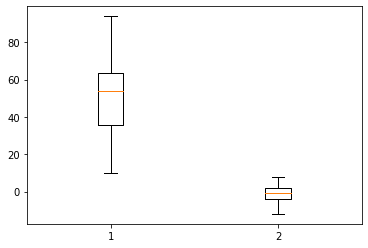
\includegraphics{fig-3-1.png}
    \end{figure}
    Očitno vidimo, da je prvi stolpec (razlika v pulzu študentov z obremenitvijo) bistveno višje od drugega (razlika v pulzu študentov brez obremenitve).

    \pagebreak
    \solution
    \begin{minted}[autogobble,breaklines]{python}
        data = sorted(list(map(lambda x: x[9] - x[8], pulz_by_load[0])))
        plt.hist(data, edgecolor='black', bins=15)
        plt.show()
    \end{minted}
    \begin{figure}[h!]
        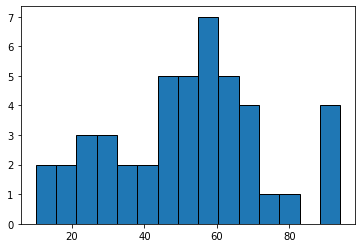
\includegraphics{fig-3-2.png}
    \end{figure}
    Ker so vse razlike pulzov študentov pod obremenitvijo večje od razlik študentov brez obremenitve, ne moremo sklepati gotovo, da je kdo goljufal,
    vendar je pa razpon razlik zelo asimetričen, kar je lahko sumljivo, če je to atipično za splošno populacijo. Če predpostavim, da pričakujemo normalno porazdelitev, potem te podatki kažejo na to, da so nekateri študentje vsaj do neke mere goljufali.
    \begin{minted}[autogobble,breaklines]{python}
        import diptest
        diptest.diptest(data)
    \end{minted}
    \begin{verbatim}
        (0.03571428571428571, 0.9609662395003099)
    \end{verbatim}
    Če opravimo Hardiganov preizkus dip, dobimo z \(96\%\) gotovostjo, da so podatki unimodalni, kar nakazuje, da do goljufanja morda ni prišlo.


    \pagebreak
    \solution
    \begin{minted}[autogobble,breaklines]{python}
        pulz_with_load_by_training = tuple(list(filter(lambda x: x[6] == i+1, pulz_by_load[0])) for i in range(3))
        data = tuple(list(map(lambda x: x[9] - x[8], pulzi)) for pulzi in pulz_with_load_by_training)
        plt.boxplot(data)
        plt.show()
    \end{minted}
    \begin{figure}[h!]
        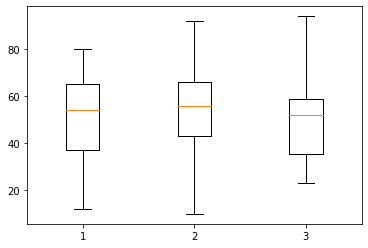
\includegraphics{fig-3-3.png}
    \end{figure}

    Podatki ne kažejo, da vadba vpliva na spremembo pulza.
\end{homeworkProblem}

\end{document}
